\documentclass[11pt]{article}

% AMS Packages
\usepackage{amsmath} 
\usepackage{amssymb} 
\usepackage{amsthm}
% Page dimensions
\usepackage[margin=1in]{geometry}
% Images
\usepackage[pdftex]{graphicx} 
% Enumerate package
\usepackage{enumitem} 
\usepackage{array} 
% Fancify pages
\usepackage{fancyhdr} 
% Convert captions on figures to bold font
\usepackage[labelfont=bf,textfont=md]{caption}
% Time New Roman font
\usepackage{times}
% change the line spacing
\usepackage{setspace} 
% SI Units in math type
\usepackage{siunitx}
% extra symbols
\usepackage{textcomp} 
\usepackage{wrapfig}
% tikz 
\usepackage{tikz}
\usetikzlibrary{shapes.geometric, arrows}
\usepackage{bm}
% Change sizes of sections
\usepackage{titlesec}
\titleformat{\section}{\normalfont\large\bfseries}{\thesection}{1em}{}
\titleformat{\subsection}{\normalfont\bfseries}{\thesubsection}{1em}{}
\titleformat{\subsubsection}{\normalfont\small\bfseries}{\thesubsubsection}{1em}{}
% Declare useful math operators
\DeclareMathOperator*{\argmin}{arg\,min}
\DeclareMathOperator*{\plim}{plim}
\DeclareMathOperator{\Tr}{Tr}
\usepackage{float}

\usepackage{algorithm}
\usepackage[noend]{algpseudocode}
\makeatletter
\makeatother

\newcommand{\varendash}[1][5pt]{%
	\makebox[#1]{\leaders\hbox{--}\hfill\kern0pt}%
}

\pagestyle{fancy}
\chead{\textbf{\small Union of Intersections (UoI) for interpretable data driven discovery and prediction in neuroscience}}
\rhead{}
\lhead{}
\headsep 5pt

% title
\title{\textbf{Union of Intersections (UoI) for for Interpretable Data Driven Discovery and Prediction in Neuroscience}}
\author{\Large Supplementary Information}
\date{}
\begin{document}
\thispagestyle{empty}
\maketitle
\section{Coupling Models}
We applied UoI$_{\text{Lasso}}$ to coupling matrices obtained from the following datasets:
\begin{itemize}
	\item \textbf{(PVC)} Single-unit activity taken from monkey primary visual cortex (Kohn et al., 2012) in response to drifting gratings.
	\item \textbf{(A1)} Micro-electrocorticography recordings taken from rat auditory cortex (Bouchard et al., 2018) in response to tone pips.
	\item \textbf{(M1/S1)} Single-unit activity taken from monkey primary motor and somatorsensory cortices (Makin et al., 2018) during reaches on a grid of targets.
\end{itemize}

Each coupling model attempted to linearly predict the activity of a target neuron (electrode) using the activities of the remaining neurons (electrodes). We fit the coupling model with Lasso and three variants of UoI$_{\text{Lasso}}$ (optimizing for $R^2$, AIC, and BIC) through a 10-fold cross-validation. We compared the models generated by each of these variants to the model obtained via Lasso. We quantified model performance by the selection ratio (fraction of non-zero parameters), explained variance ($R^2$), Akaike Information Criterion, and the Bayesian Information Criterion. The two information criterions are defined as
\begin{align}
	\text{AIC} &= 2k - 2 \log(\hat{L}) \label{eqn:aic}\\
	\text{BIC} &= \log(n) \cdot k - 2 \log(\hat{L}) \label{eqn:bic}
\end{align}
where $\log(\hat{L})$ is the log-likelihood of the model on the test set, $n$ is the number of test samples, and $k$ is the number of features. In contrast to explained variance, lower information criterion is preferable. Thus, AIC and BIC penalize models with larger numbers of parameters (first term in equations \ref{eqn:aic} and \ref{eqn:bic}). In addition, the BIC generally prefers sparser models more strongly than the AIC.
\subsection{PVC}
This dataset was recorded by Matthew Smith and Adam Kohn and obtained through the pvc-11 dataset from CRCNS. Spiking activity was recorded from V1 in three anesthetized macaque monkeys during presentations of drifting gratings. Single-unit spiking responses were segmented into trials according to stimulus presentation. In total, there were 2400 trials recorded with 3 monkeys, each with 106, 88, and 112 single-units, respectively.

We caculated each response variable as the square-root of the spike count in the trial. Thus, the coupling model predicts whether the (square-rooted) spike count in a given trial can be described linearly by the (square-rooted) spike counts according to the remaining neurons in the population. The performance of Lasso compared to the three variants of UoI$_{\text{Lasso}}$ is depicted in Figure \ref{fig:pvc} for each monkey. We observe that UoI$_{\text{Lasso}}$ provides sparser models (top row) at limited or no cost to predictive power (second row) resulting in improved information criterion scores (bottom two rows; recall that lower information criterion is better). In addition, the three variants of UoI$_{\text{Lasso}}$ prefer different levels of sparsity, with $UoI_{\text{Lasso}}-$BIC resulting in the sparsest models.


\begin{figure}[t]
	\centering
	\scalebox{0.24}{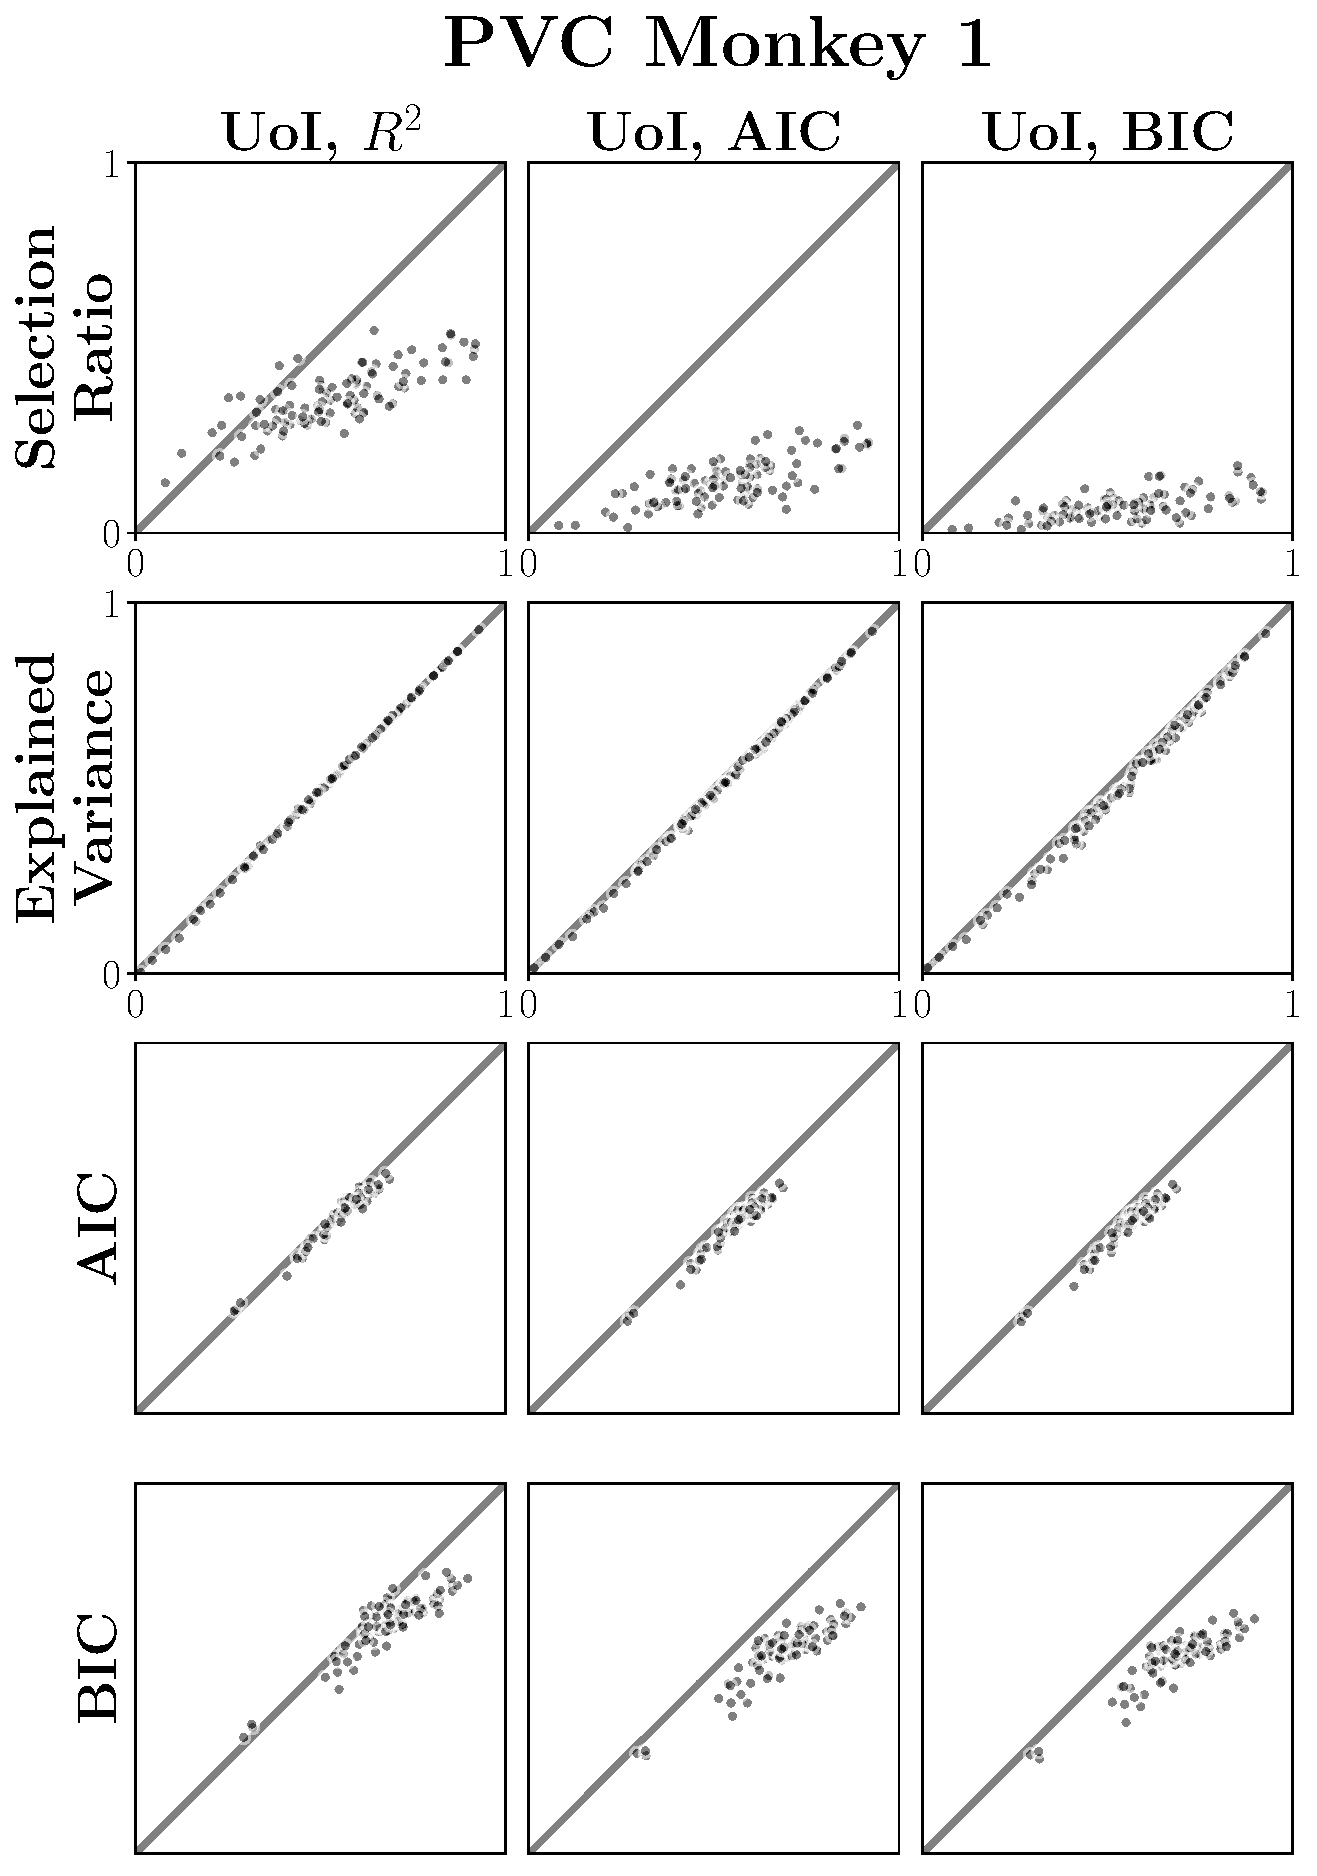
\includegraphics{img/coupling/pvc11_monkey1.pdf}}
	\scalebox{0.24}{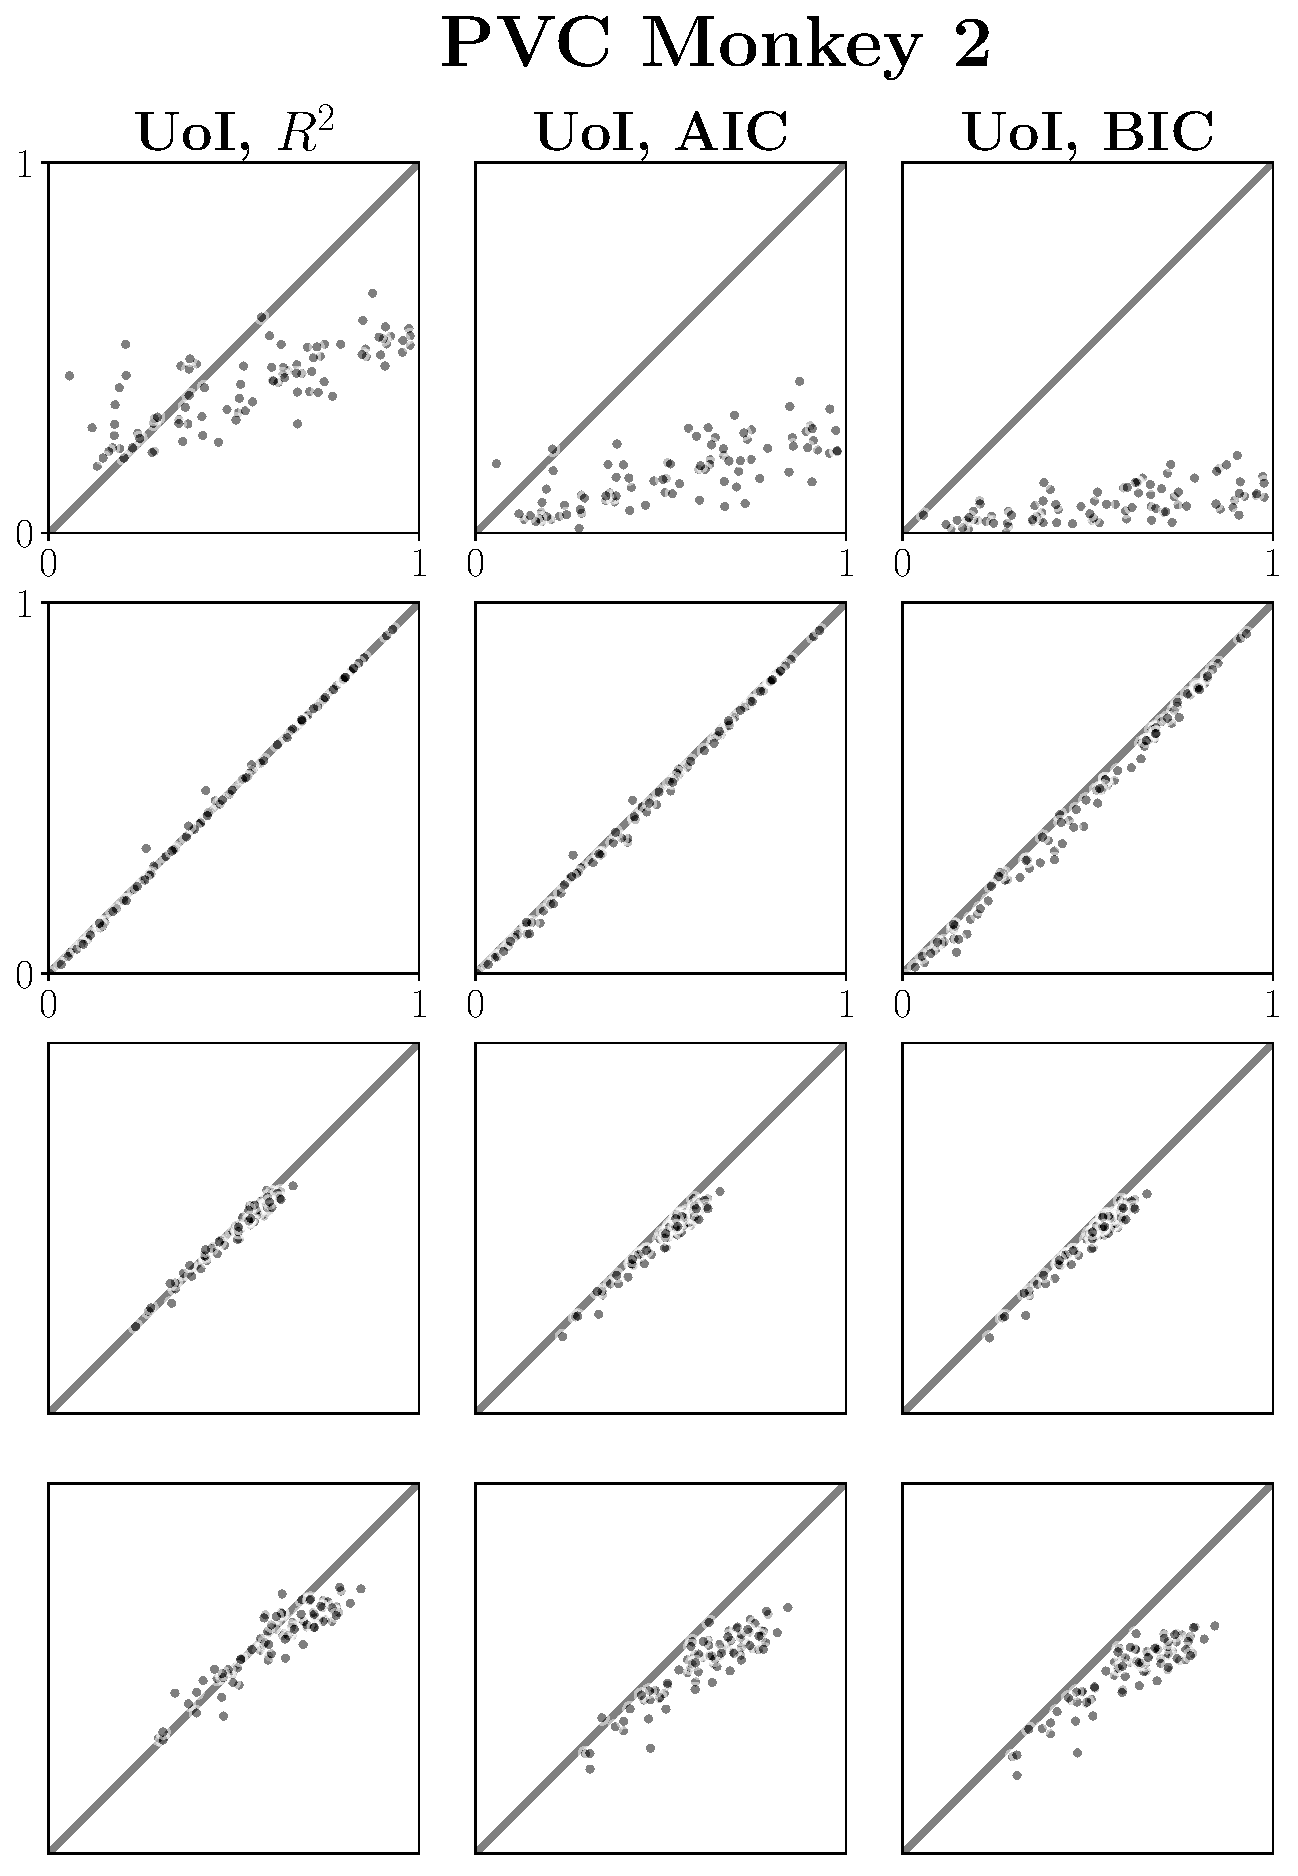
\includegraphics{img/coupling/pvc11_monkey2.pdf}}
	\scalebox{0.24}{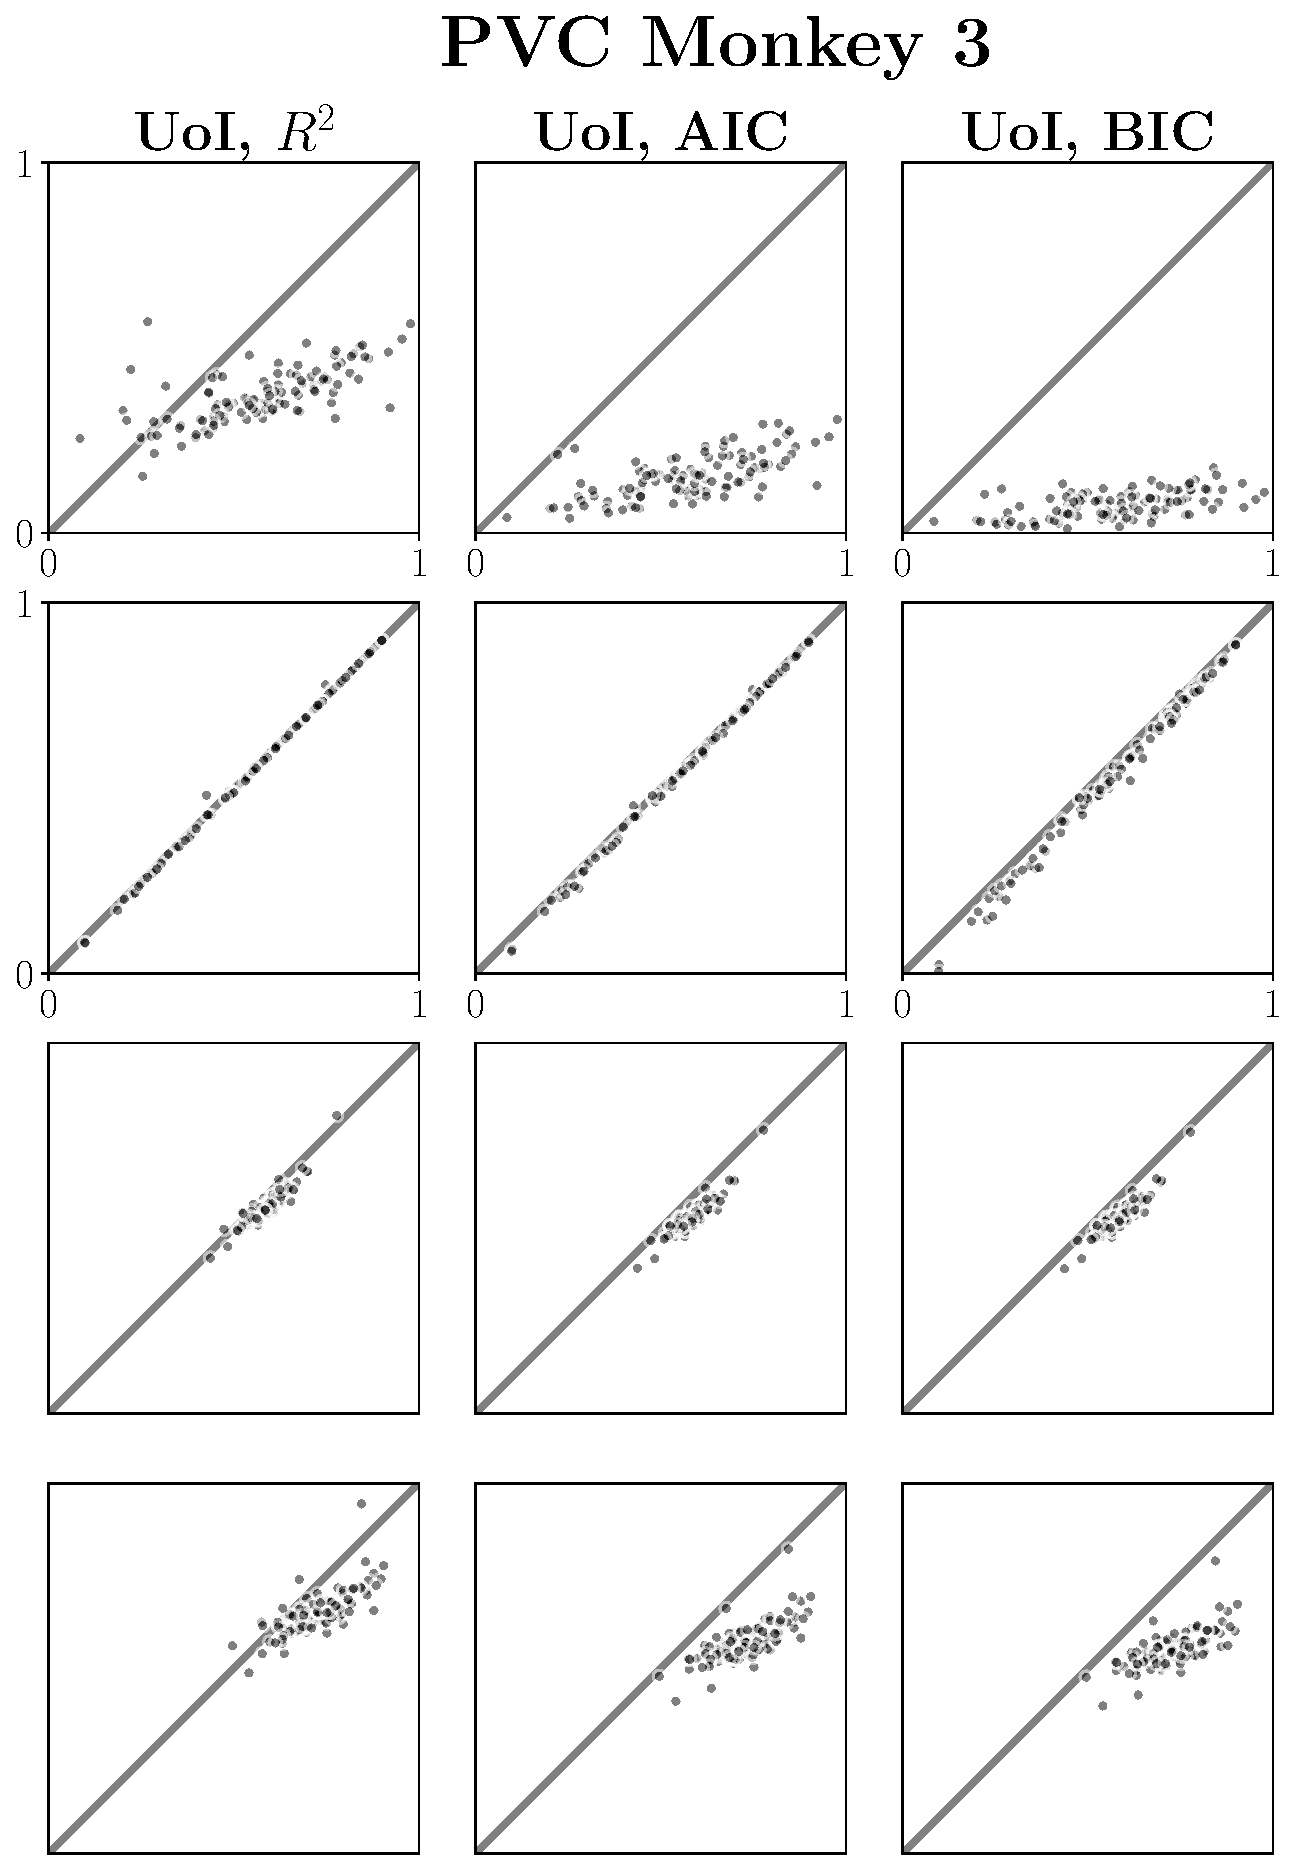
\includegraphics{img/coupling/pvc11_monkey3.pdf}}

	\caption{Lasso ($x$-axis) vs. the three variants of UoI$_{\text{Lasso}}$ ($y$-axes) on Monkey 1 (Left), Monkey 2 (Center), and Monkey 3 (Right). Metrics considered are, in order of rows, selection ratio (number of non-zero parameters divided by total possible number of parameters), explained variance ($R^2$), Akaike Information Criterion, and the Bayesian Information Criterion.}
	\label{fig:pvc}
\end{figure}


\subsection{A1}
\begin{wrapfigure}{r}{0.35\textwidth}
	\vspace{-60pt}
	\centering
	\scalebox{0.26}{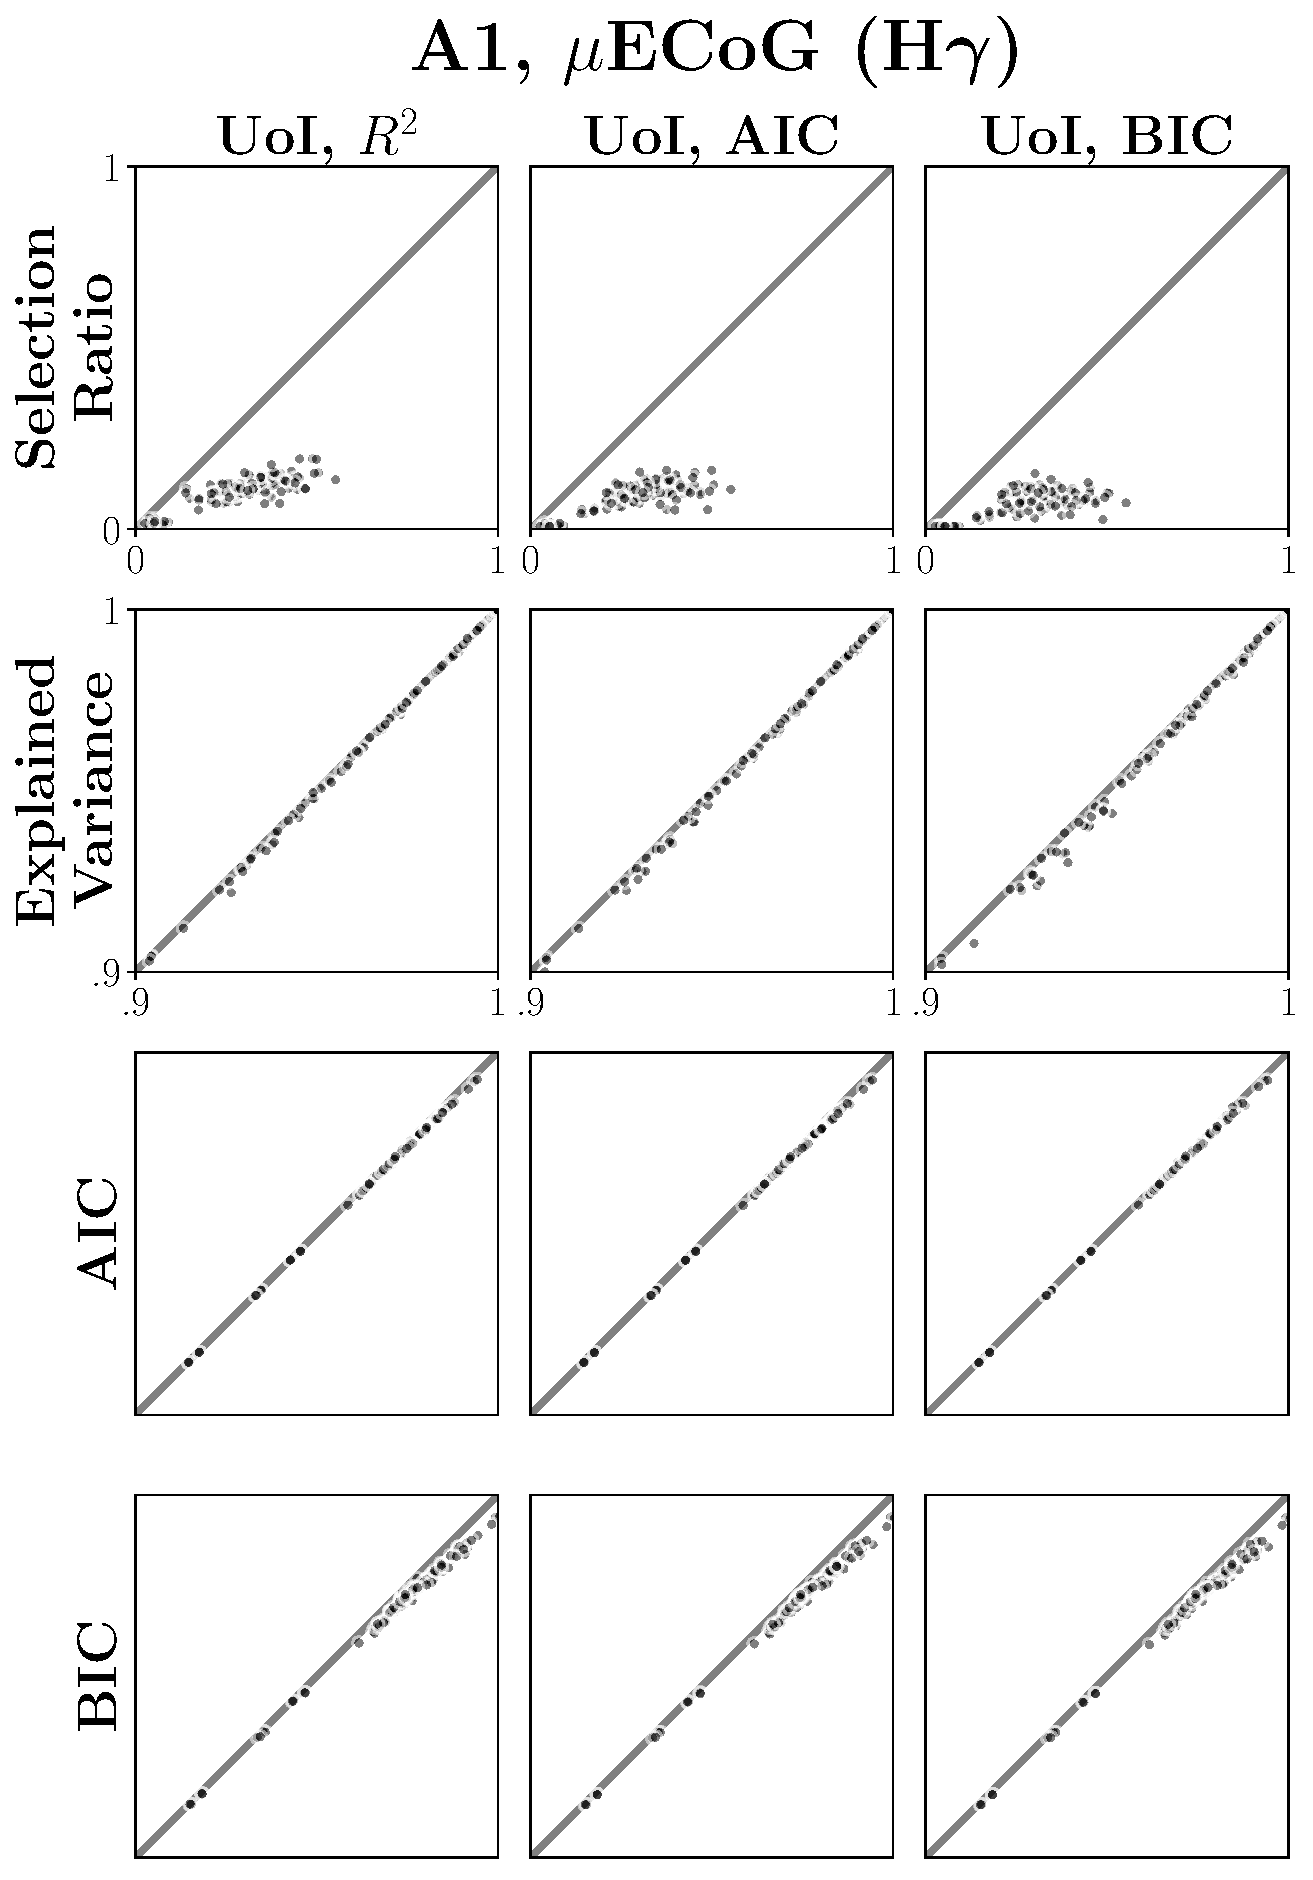
\includegraphics{img/coupling/ecog_HG.pdf}}
	\caption{Lasso ($x$-axis) vs. the three variants of UoI$_{\text{Lasso}}$ ($y$-axes) on rat auditory cortex coupling models. Rows are metrics while columns are variants of UoI$_{\text{Lasso}}$.}
	\label{fig:ecog}
\end{wrapfigure}
This dataset was recorded by the Bouchard Lab (the specific rat was R32-B7). Micro-electrocorticography was performed on the surface of the auditory cortex in anesthetized rats during the presentation of tone pips at varying frequencies and attenuations. The $\mu$ECoG recordings were  $z$-scored relative to baseline before stimulus presentation and segmented into trials based on the stimulus type. There were 4200 trials (30 frequencies, 7 attenuations, and 20 repetitions) and 128 electrodes. 

We calculated each response variable as the peak response of the $z$-scored high-gamma analytic amplitude. Thus, the coupling model predicts whether the peak response in a given trial can be described linearly by the peak responses of the remaining electrodes. A comparison of Lasso to the variants of UoI$_{\text{Lasso}}$ are shown in Figure \ref{fig:ecog}. Note that the explained variance plots cover the range $[0.9, 1.0]$, since the coupling models were highly predictive. UoI$_{\text{Lasso}}$ resulted in considerably sparser models coming at little to no cost to explained variance.  Similarly to the previous Figure, we observe that there is a spectrum of enforced sparsity, with UoI$_{\text{Lasso}}$--BIC providing the sparsest models. For this dataset, UoI$_{\text{Lasso}}$--AIC provides a good balance between sparsity and predictive power.

\subsection{M1}
\begin{wrapfigure}{r}{0.35\textwidth}
	\vspace{-25pt}
	\centering
	\scalebox{0.26}{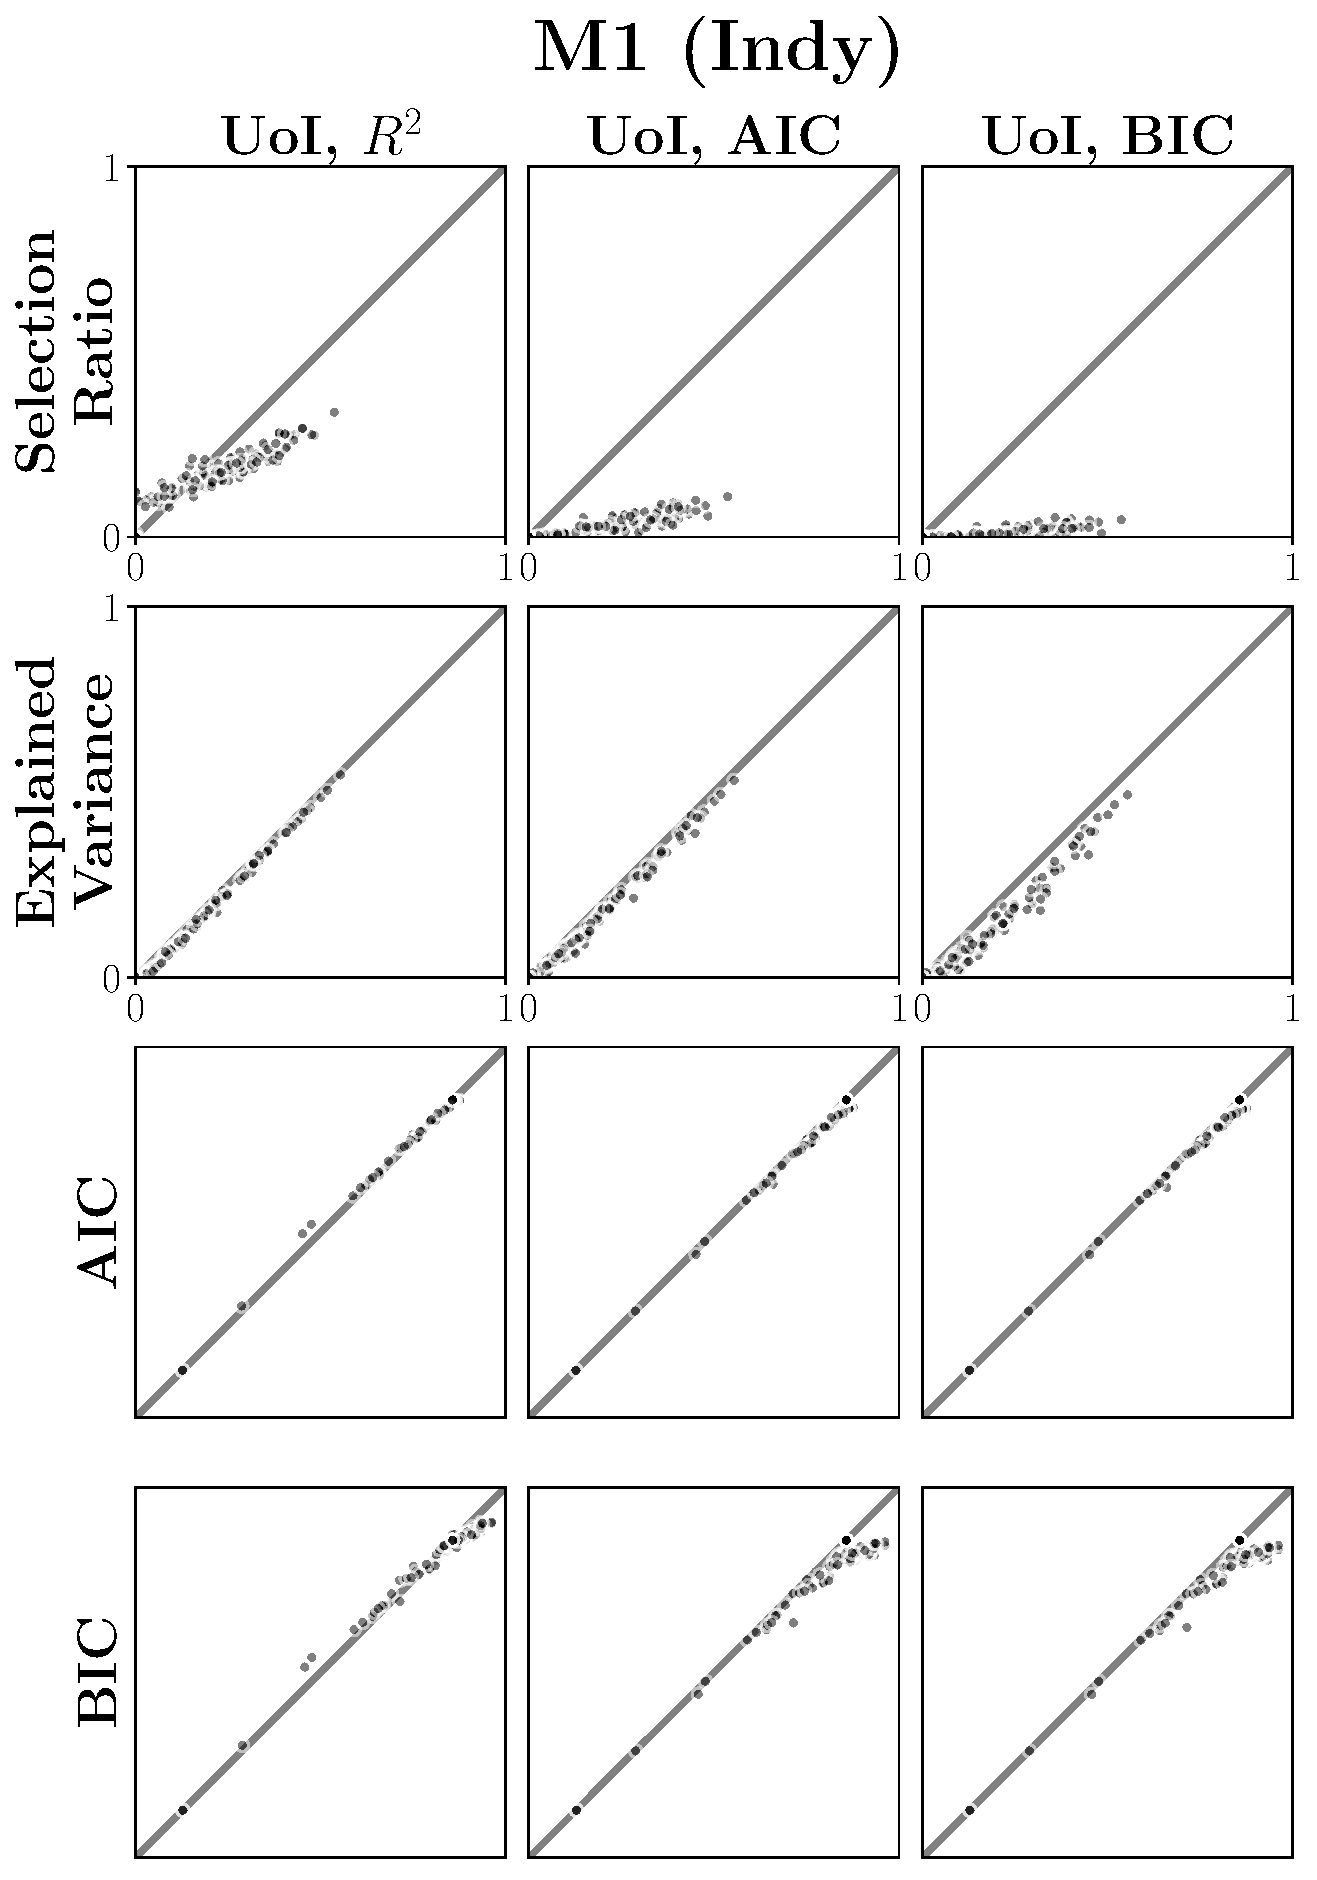
\includegraphics{img/coupling/nhp_indy_20160411_01.pdf}}
	\caption{Lasso ($x$-axis) vs. the three variants of UoI$_{\text{Lasso}}$ ($y$-axes) on nonhuman primate coupling models.}
	\label{fig:nhp}
\end{wrapfigure}
This dataset was recorded by the Sabes Lab (obtained through Zenodo). Single-unit responses were obtained from non-human primate primary motor cortex during self-paced reaches to target on a grid. The primate was prompted to reach for a specific target without gaps or pre-movement delay intervals. We binned the total spike trains for all the recorded single-units to widths of 500 milliseconds. According to this binning, there were 1716 samples for 196 single-units.

We caculated each response variable as the square-root of the spike count in the bin. Thus, the coupling model predicts whether the (square-rooted) spike count in a given bin can be described linearly by the (square-rooted) spike counts according to the remaining neurons in the population. 

The performance of Lasso compared to the three variants of UoI$_{\text{Lasso}}$ is depicted in Figure \ref{fig:nhp} for a given primate (Indy) and session (04-11-2016-1). Interestingly, UoI$_{\text{Lasso}}$ provides sparser models except for a subset of neurons under the UoI$_{\text{Lasso}}-R^2$ variant. However, UoI$_{\text{Lasso}}$ still maintains predictive performance, resulting in simpler but predictive models.\\

\newpage

\section{Tuning}
\subsection{A1}

\begin{wrapfigure}{r}{0.35\textwidth}
	\vspace{-40pt}
	\centering
	\scalebox{0.26}{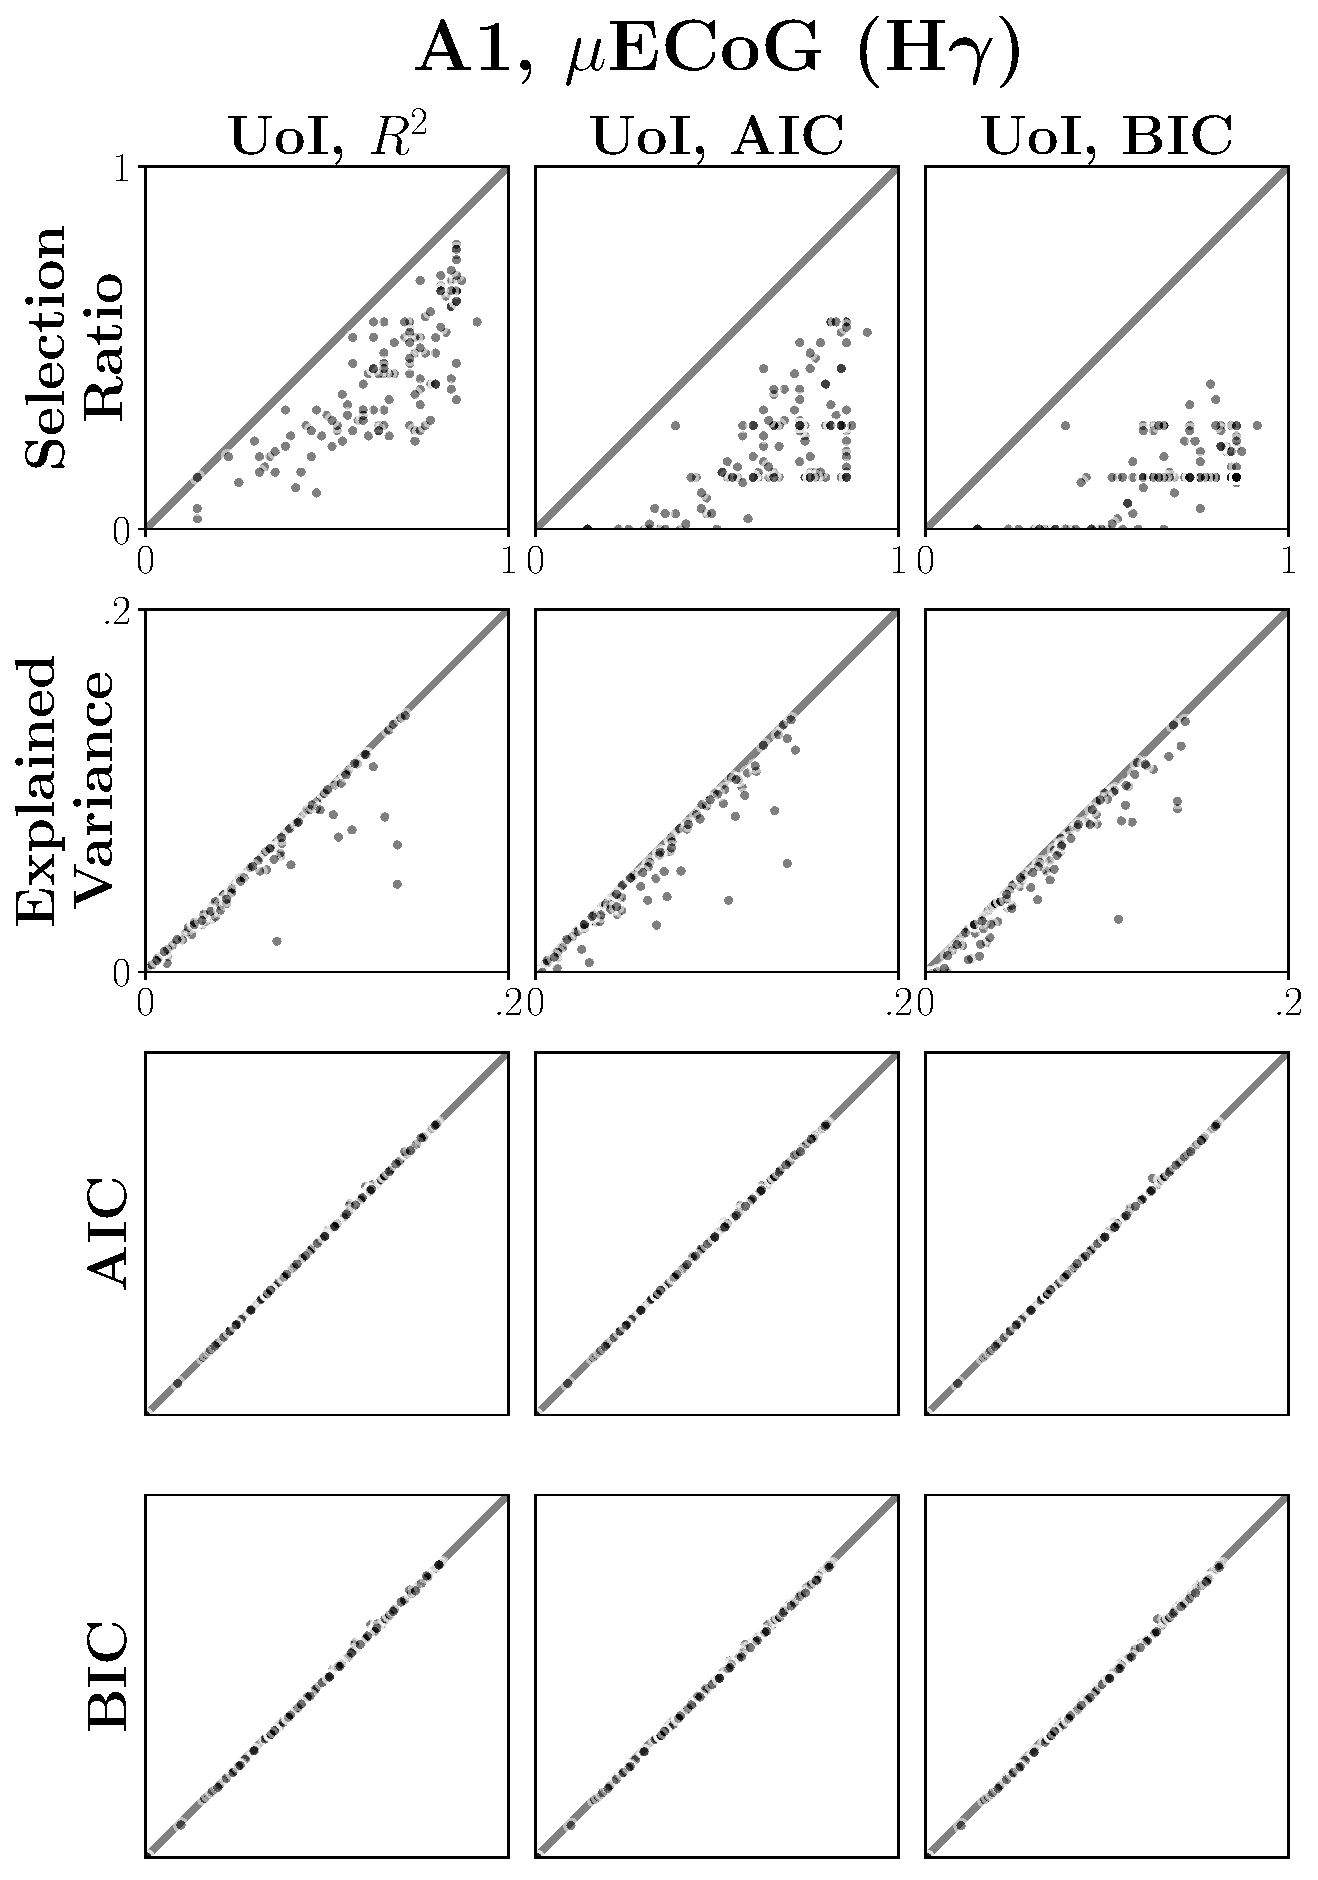
\includegraphics{img/tuning/ecog_hg.pdf}}
	\caption{Lasso ($x$-axis) vs. the three variants of UoI$_{\text{Lasso}}$ ($y$-axes) for auditory tuning data.}
	\label{fig:ecog_tuning_scores}
	\vspace{-30pt}
\end{wrapfigure}
We fit tuning curves to the auditory $\mu$ECoG recordings using Gaussian basis functions tiling the log-frequency axis. Specifically, the response $y_i$ for a given electrode was modeled as
\begin{align}
y_i(f) &= a_0 + \sum_{j=1}^k a_j \exp\left(-\frac{(f - f_j)^2}{2\sigma_i^2}\right)
\end{align}
where $f_j$ are spread evenly in log-frequency, $k$ is the number of Gaussians (features), and $\sigma_i$ is the spread of the Gaussian basis functions, generally chosen uniformly across all electrodes. The relevant tuning parameters to be fit are the $a_j$. For the $\mu$-ECoG data, we used 7 Gaussians spread evenly from  0.5 to 32 kHz, and $\sigma_i^2=0.64$ octaves. We fit this model using Lasso and the UoI$_{\text{Lasso}}$ variants.

The model performance is shown in Figure \ref{fig:ecog_tuning_scores}. Note that the maximum number of features that can be used is 7, so differences in selection ratio denote a difference in only a few features. In this case, UoI$_{\text{Lasso}}-R^2$ uses fewer features to achieve the same predictive performance for almost all electrodes. There is little different in the information criteria because the number of features is small compared to the amount of data.

In addition, we also examined tuning curves across the $\mu$ECoG grid. The curves are shown in Figure \ref{fig:ecog_tuning_curves}, plotted against log-frequency. Lasso and UoI$_{\text{Lasso}}$ generally agree on almost all electrodes. Both fitting procedures result in broad tonotopy across the grid. For some electrodes, UoI$_{\text{Lasso}}-$BIC (dashed red) zeros out all coefficients except the intercept. In these cases, the penalty for requiring parameters is greater than the relatively weak model performance (observe the scale in Figure \ref{fig:ecog_tuning_scores}).
\begin{figure}[b!]
	\centering
	\scalebox{0.435}{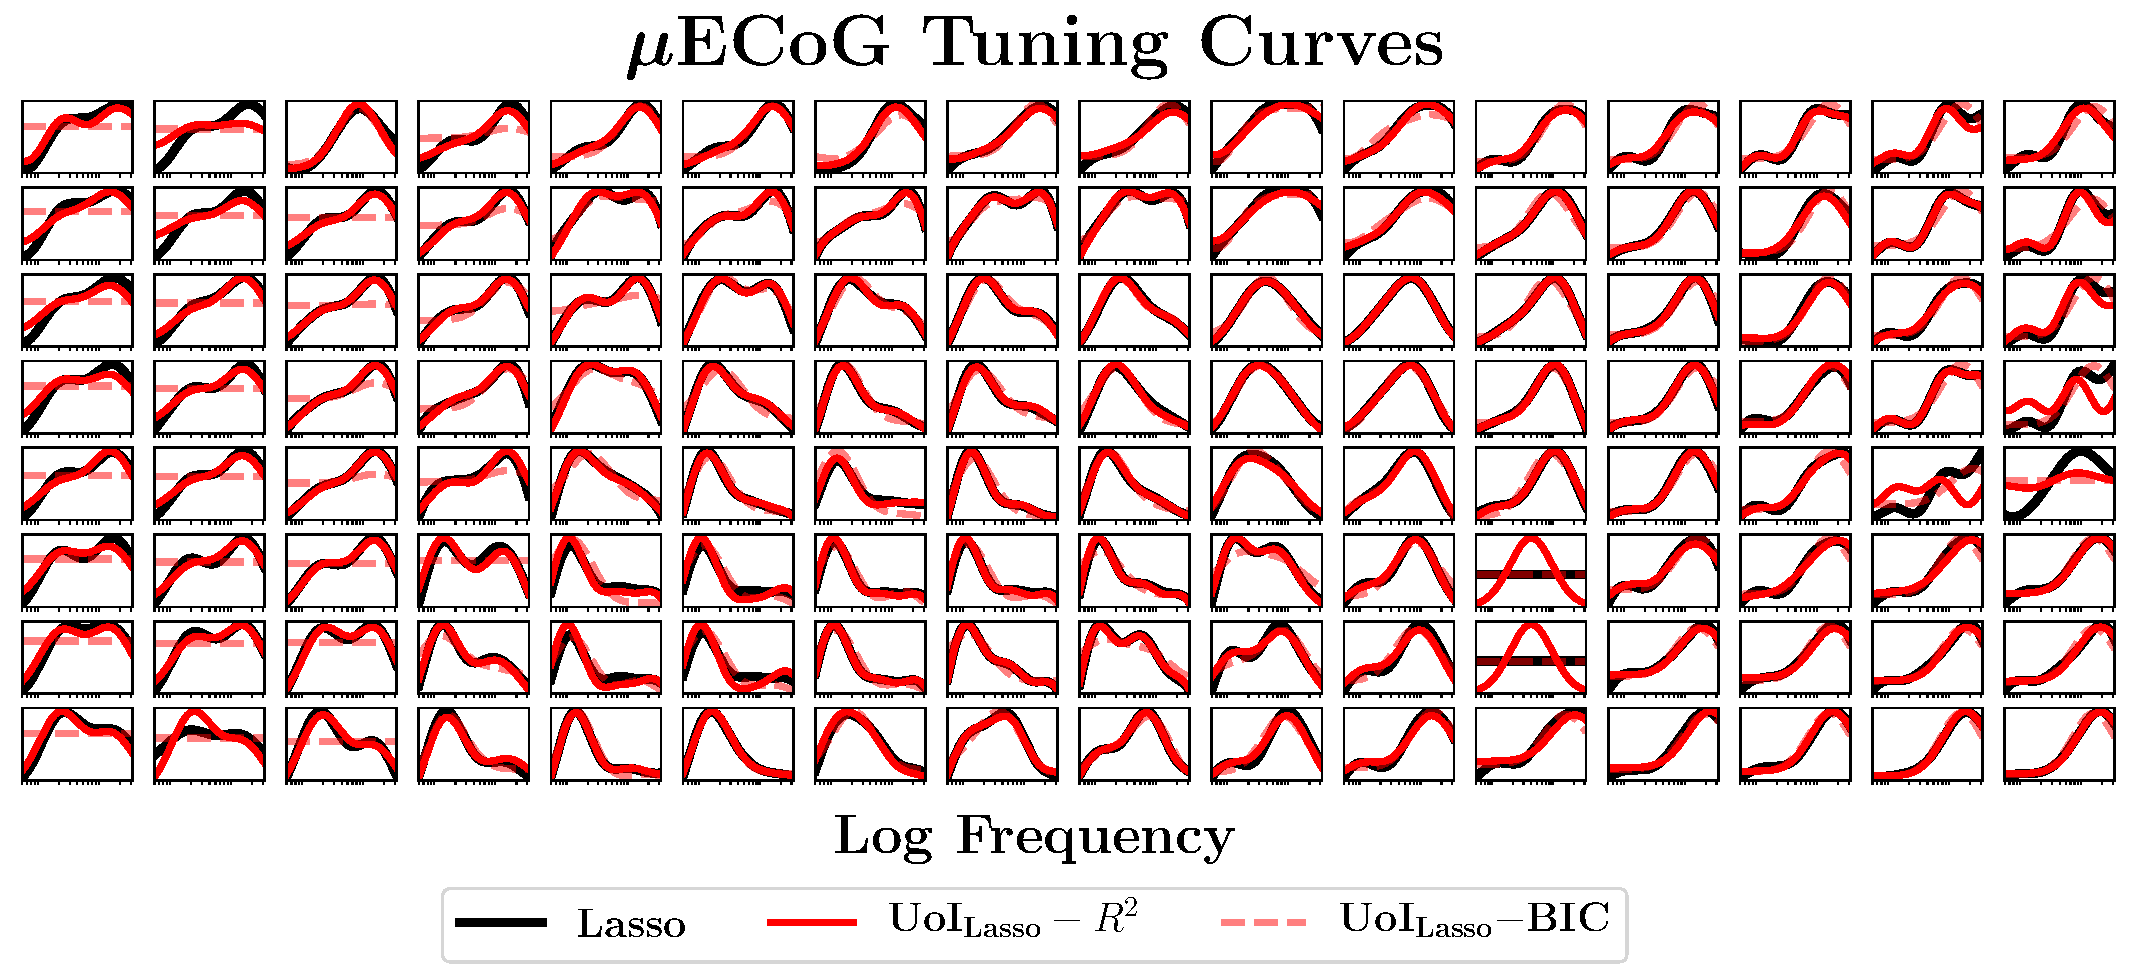
\includegraphics{img/tuning/ecog_grid.pdf}}

	\caption{Auditory tuning curves plotted against log-frequency for each electrode on the $\mu$ECoG grid. Three separate fits are shown: Lasso (black), UoI$_{\text{Lasso}}-R^2$ (red) and UoI$_{\text{Lasso}}-$BIC (dashed red).}
	\label{fig:ecog_tuning_curves}
\end{figure}

\section{Classification}
\subsection{Recordings from Basal Ganglia}
We consider a dataset from the Berke lab involving recordings from the basal ganglia of rats. Specifically, these datasets are taken from the  globus pallidus (GP) and substantia nigra pars reticulata (SNr). These regions generally participate in race pathways during decision making. The task that allowed the experimenters to assess these pathways is as follows:
\begin{itemize}
	\item A rat is prompted to enter its head in one of three ports using a visual cue. 
	\item Once the rat has placed its head through the port, it is then prompted, with a tone, to either go to the left port or right port. The frequency of the tone indicates whether it should be left or right (GO condition).
	\item On some fraction of the trials, the direction tone will be followed by a white noise burst, indicating that the rat should remain in the center port (STOP condition).
	\item In some trials, the rat moves before the GO tone occurs, which is considered a pre-tone failure.
\end{itemize}
Thus, there are several decisions that can be predicted based on the neural recordings:
\begin{itemize}
	\item Can we predict whether the rat made a pre-tone error according to the neural activity? (432 trials, 18/36 features).
	\item Can we predict whether the trial was a GO or STOP trial based on the neural activity? (326 trials, 18/36 features).
	\item Can we predict whether the trial was a left or right GO trial based on the neural activity? (186 trials, 18/36 features).
\end{itemize}

\subsection{Prediction of pre-tone failure}
We used neural activity to predict whether a rat would fail on a trial pre-tone. Specifically, we examined spike counts of the 18 units in GP in a timespan following the point when the rat enters the center port. The delays between the trials on which the rat failed pre-tone and succeeded pre-tone had different lengths of time between the rat entering and exiting the center port (Figure \ref{fig:classification}, left). 

\begin{figure}[b]
	\centering
	\includegraphics[scale=0.40]{img/classification/delay.pdf}
	\includegraphics[scale=0.40]{img/classification/gp1.pdf}
	\caption{\textbf{Left:} Time between center-in and center-out for pre-tone failures (red) and successes (blue). \textbf{Right:} Prediction accuracy by fitted logistic regression model on validation set (5 folds). Red line is chance (only predicting pre-tone success).}
	\label{fig:classification}
\end{figure}

We examined the spike counts in the period $(C_0, C_0 + \Delta t)$ where $C_0$ is the center-in time of the rat and $\Delta t \in \left\{0.1, 0.2, \ldots 1.0 \right\}$. We used a logistic regression model with the spike counts of each neuron as the predictors, and the pre-tone success/failure as the response. In Figure \ref{fig:classification}, right, we show the test set performance of the model across the 5-folds during cross-validation over the different values of $\Delta t$. There appears to be no strong modulation in the classifier performance, and it performs marginally better than if it had always selected pre-tone success (red line).

Lastly, we examined the coefficients of the logistic regression models as a function of $\Delta t$. The coefficients were somewhat sparse (4/18 features were consistently set to zero). Furthermore, the remaining coefficients were relatively stable for different values of $\Delta t$ (Figure 7).

\begin{figure}[h]
	\centering
	\includegraphics[scale=0.40]{img/classification/coefs.pdf}
	\caption{Median coefficient values as a function of $\Delta t$ for the 18 well isolated units.}
	\label{fig:classification}
\end{figure}
\end{document}
